\documentclass[a4paper, 11pt]{article}
\usepackage{covington}
\usepackage{amssymb}
\usepackage{amsmath}
\usepackage[catalan]{babel}
\usepackage{graphicx}
\usepackage{eurosym}
\usepackage{caption}
\usepackage{subcaption}
\usepackage{float}
\usepackage{bm}
\usepackage{layout}
\usepackage{hyperref}
\textheight=23.94cm 
\textwidth=17cm 
\topmargin=-1cm 
\oddsidemargin=-0.5cm 
 
\newcommand{\header}[4]{
	\begin{center}
		\rule{\linewidth}{0.5pt}
		
		{\small{#1}}
      
        \vspace{0.2in}
        
		{\large{#2}}
		
        \vspace{0.2in}
        
		{\small{#3}}
		
		\vspace{0.15in}
		
		{#4}
		
		\vspace{-0.1in}
		\rule{\linewidth}{0.6pt}
	\end{center}
}

\begin{document}
 
\header{\sc Barcelona Graduate School of Economics \hfill Master's Degree in Data Science}{\bf Statistical Modeling and Inference $-$ Problem Set \#6}{\sc Group 3: Niti Mishra $\cdot$ Miquel Torrens $\cdot$ B\'alint V\'an}{November 30\textsuperscript{th}, 2015}
Solution to proposed exercises.\\
% EXERCISE 1
\newline \textbf{\underline{Exercise 1}}\\
\newline \underline{Part (a)}\\
\newline Given $t_n \sim \text{Laplace}(\mu, \Lambda)$, the likelihood function is:
\begin{eqnarray}
\mathcal{L} (\text{Laplace} (t_n | \mu, \Lambda)) = \prod_{n=1}^{N} f(t_n | \mu, \Lambda) = \left(  \frac{\Lambda}{2} \right)^N \exp \left\{ -\Lambda \sum_{n=1}^{N} | t_n - \mu | \right\} \nonumber
\end{eqnarray}
\newline \underline{Part (b)}\\
\newline If we take the MLE:
\begin{eqnarray}
\max_{\mu, \Lambda} \log \mathcal{L} = \max_{\mu, \Lambda} N \log \Lambda - \Lambda  \sum_{n=1}^{N} | t_n - \mu | + C  \nonumber
\end{eqnarray}
With $C$ containing the terms not dependent on $\mu$ or $\Lambda$. Then:
\begin{eqnarray}
\frac{\partial \log \mathcal{L}}{\partial \mu} = 0 &\Leftrightarrow& - \Lambda \sum_{n=1}^{N} \frac{ t_n - \mu }{| t_n - \mu |} = 0 \nonumber \\
&\Leftrightarrow& \sum_{n=1}^{N} \text{sgn}(t_n - \mu_{MLE}) = 0 
\end{eqnarray}
Note that with odd $N$, for (1) to hold, $(N-1)/2$ observations need to have $t_n \geq \mu$ and $(N-1)/2$ have $t_n \leq \mu$. The unpaired observation will have $t_n = \mu$. Thus:
\begin{eqnarray}
\mathbb{E}[t] = \mu_{MLE} = \text{median}(t_1, t_2, ..., t_n) \nonumber
\end{eqnarray}
is the expected value and also the median.\\
\newline \underline{Part (c)}\\
\newline We derive $\Lambda_{MLE}$:
\begin{eqnarray}
\frac{\partial \log \mathcal{L}}{\partial \Lambda} = 0 &\Leftrightarrow& N \frac{1}{\Lambda} - \sum_{n=1}^{N} | t_n - \mu | = 0 \nonumber \\
&\Leftrightarrow& \Lambda_{MLE} = \left( \frac{1}{N} \sum_{n=1}^{N} | t_n - \mu | \right)^{-1}  \nonumber
\end{eqnarray}
\newline \underline{Part (d)}\\
\newline By the equivariance property\footnote{Wasserman's Theorem 10.14.} of the MLE:
\begin{eqnarray}
\text{var}[t] = \Sigma_{MLE} = \frac{2}{\Lambda_{MLE}^2} = 2 \left( \frac{1}{N} \sum_{n=1}^{N} | t_n - \mu | \right)^2. \nonumber
\end{eqnarray}
% EXERCISE 2
\newpage
\textbf{\underline{Exercise 2}}\\
\newline \underline{Part (a)}\\
\newline Given:
\begin{eqnarray}
t_n \sim \mathcal{N}(t_n | \mathbf{x}_n, \mathbf{w}, \eta_n, q) = \frac{(\eta_n q)^{1/2}}{\sqrt{2 \pi}} \exp \left\{ - \frac{\eta_n q}{2} (t_n - \phi(\mathbf{x}_n) \mathbf{w})^T (t_n - \phi(\mathbf{x}_n) \mathbf{w} ) \right\}  \nonumber
\end{eqnarray}
and:
\begin{eqnarray}
\eta_n \sim \text{Gam} \left(\eta_n | \frac{\nu}{2}, \frac{\nu}{2} - 1 \right) = \frac{\left( \frac{\nu}{2} - 1 \right)^{\nu/2}}{\left(\frac{\nu}{2} - 1 \right)!} \eta_n^{\left(\frac{\nu}{2} - 1 \right)} \exp \left\{ - \left(\frac{\nu}{2} - 1 \right) \eta_n \right\}   \nonumber
\end{eqnarray}
We know:
\begin{eqnarray}
p(\eta_n | t_n, \mathbf{x}_n, \mathbf{w}, q) &\propto& p(t_n | \eta_n, \mathbf{x}_n, \mathbf{w}, q) p(\eta_n)  \nonumber \\
&=& C \eta_n^{(\frac{\nu}{2} - 1 + \frac{1}{2})} \exp \left\{ - \left( \frac{\nu}{2}-1 \right) \eta_n - \frac{\eta_n q}{2} \mathbf{e}_n^T \mathbf{e}_n \right\} \nonumber \\
&=& C \eta_n^{(\frac{\nu + 1}{2} - 1)} \exp \left\{ \left( - \left( \frac{\nu}{2}-1 \right) - \frac{q}{2} \mathbf{e}_n^T \mathbf{e}_n \right) \eta_n \right\} \nonumber \\
&=& C \eta_n^{(\frac{\nu + 1}{2} - 1)} \exp \left\{ - \left( \frac{\nu + q \mathbf{e}_n^T \mathbf{e}_n}{2} - 1 \right) \eta_n \right\} \nonumber
\end{eqnarray}
Where $C$ contains the multiplication of the terms of the density functions not dependent on $\eta_n$. Observe this is a Gamma distribution with parameters:
\begin{eqnarray}
\alpha_n &=& \frac{\nu + 1}{2} \nonumber \\
\beta_n &=& \frac{\nu + q \mathbf{e}_n^T \mathbf{e}_n}{2} - 1 \nonumber
\end{eqnarray}
This finishes the proof.\\
\newline \underline{Part (b)}\\
\newline Given\footnote{Equations (4.3) and (4.4) in the \href{http://www.econ.upf.edu/~omiros/notes2005.pdf}{lecture notes} on the appendix of the lecture.}:
\begin{eqnarray}
Q(\theta, \theta') = \int \log \left( p(t, \eta | \theta) \right) p(\eta | t, \theta') d\eta = \mathbb{E}\left[ \log \left( p(t, \eta | \theta) \right) \right] \nonumber
\end{eqnarray}
We can use $\theta = (q, \mathbf{w})$ and through maximum likelihood compute:
\begin{eqnarray}
\mathbb{E}\left[ \log p(t, \eta | \theta) \right] &=& \mathbb{E}\left[ \log \left( p(t | \theta) p(\eta | t, \theta') \right) \right] \nonumber \\
&=& \mathbb{E}\left[ \log p(t | \theta) +\log p(\eta | t, \theta') \right] \nonumber \\
&=& \mathbb{E}\left[ \log \left( \prod_{n=1}^{N} \left( \frac{q \eta_n}{2 \pi} \right)^{\frac{1}{2}} \exp \left\{ -\frac{1}{2} q e_n^2 \eta_n \right\}  \right) +\log p(\eta | t, \theta') \right] \nonumber \\
&=& \mathbb{E}\left[ \log \left( \prod_{n=1}^{N} \left( \frac{q \eta_n}{2 \pi} \right)^{\frac{1}{2}} \exp \left\{ -\frac{1}{2} q e_n^2 \eta_n \right\}  \right)  \right] + \mathbb{E}\left[ \log p(\eta | t, \theta') \right] \nonumber \\
&=& \mathbb{E}\left[ \log \left( \left( \frac{q \eta_n}{2 \pi} \right)^{\frac{N}{2}} \exp \left\{ -\frac{1}{2} q \sum_{n=1}^{N} e_n^2 \eta_n \right\}  \right) \right] + c \nonumber \\
&=& \mathbb{E}\left[ \frac{N}{2} \log q - \frac{q}{2} \sum_{n=1}^{N} (t_n - \phi(\mathbf{x}_n) \mathbf{w})^2 \eta_n \right] + c \nonumber \\
&=& \frac{N}{2} \log q - \frac{q}{2} (\mathbf{t} - \mathbf{\Phi} \mathbf{w})^T \mathbb{E}\left[ \mathbf{H} \right] (\mathbf{t} - \mathbf{\Phi} \mathbf{w}) + c \nonumber
\end{eqnarray}
Where $\mathbf{H}$ is a diagonal matrix with $\mathbf{H}_{nn} = \eta_n$, and $c$ contains all terms not dependent on $\theta$. The distribution of $\eta_n$ will not depend on $\theta$ but on the previous $\theta' = (q', \mathbf{w}')$, and given that for $t \sim \text{Gam}(\alpha, \beta)$ we have $\mathbb{E}[t] = \alpha / \beta$, then:
\begin{eqnarray}
\mathbb{E}[\eta_n] = \frac{\frac{\nu + 1}{2}}{ \frac{\nu + q' (e_{n}^{'})^2}{2} - 1} = \frac{\nu + 1}{\nu + q' (e_{n}^{'})^2 - 2} = \frac{\nu + 1}{\nu + q' (t_n - \phi(\mathbf{x}_{n}) \mathbf{w}^{'})^2 - 2} \nonumber
\end{eqnarray}
Hence proved.
% EXERCISE 3
\newpage
\textbf{\underline{Exercise 3}}\\
\newline \underline{Part (a)}\\
\begin{center}
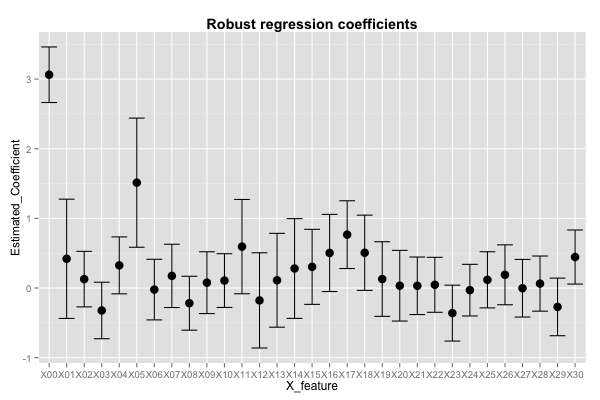
\includegraphics[scale=0.5]{ps6_plot1_1.png}\\
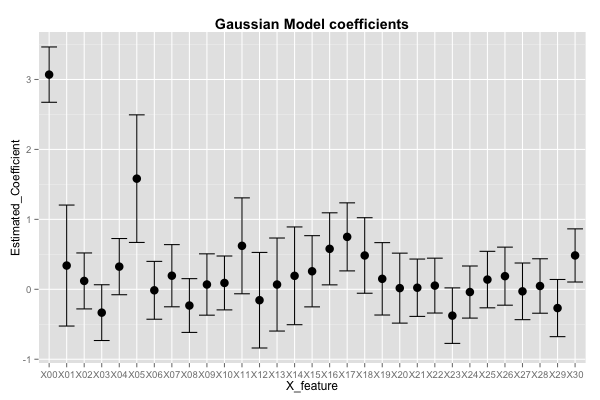
\includegraphics[scale=0.5]{ps6_plot1_2.png}
\end{center}
\underline{Part (b)}\\
\newline For completeness, we plot the values including the deviance constant terms. The residuals resemble in both models and the simulations produce very similar 99\% quantiles, though not exact. This indicates that with high probability the input data is indeed Gaussian.
\begin{center}
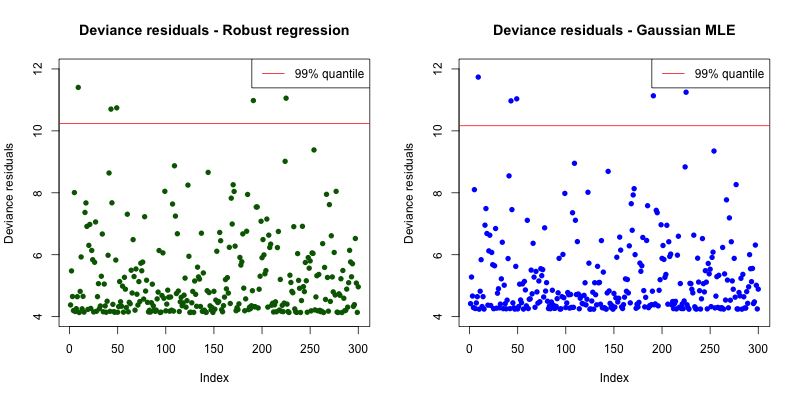
\includegraphics[scale=0.6]{ps6_plot2.png}
\end{center}
\underline{Part (c)}\\
\newline We can decide to stop the EM algorithm when the values for the estimated parameters $\theta$ estabilize, which is very similar to saying when the log-likelihood stops increasing (the sequential iterations increase its value by a very small number, say $10^{-6}$).\\
\newline Example (parameter stabilization: $q$ and $\mathbf{w}$, here only $w_1$ for illustration):
\begin{center}
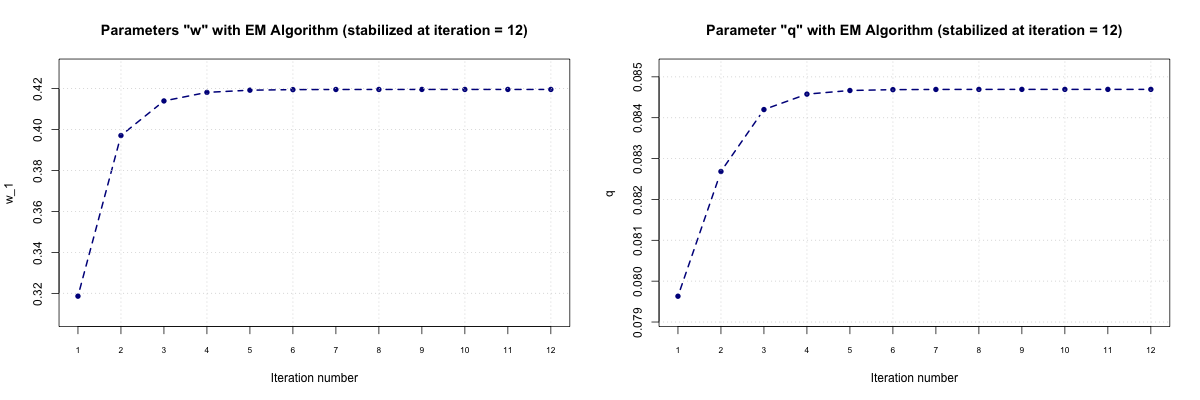
\includegraphics[scale=0.4]{ps6_plot3.png}
\end{center}
Example (log-likelihood stabilization):
\begin{center}
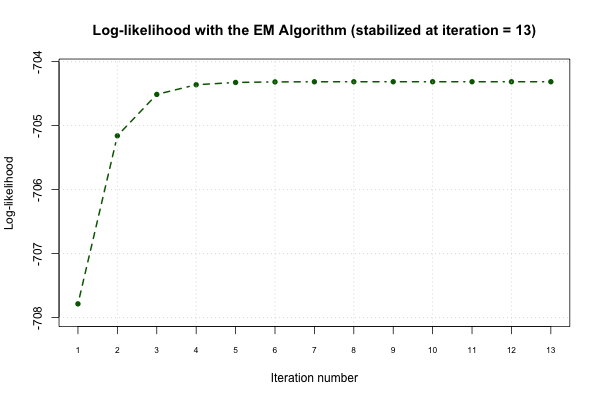
\includegraphics[scale=0.65]{ps6_plot4.png}
\end{center}
\underline{Part (d)}\\
\newline We can choose $\nu$ by running the EM algorithm for different values of $\nu$ and then choosing the smallest $\nu$ that maximizes the log-likelihood, i.e. the one for which increasing $\nu$ raises log-likelihood by a reasonably small amount, here we use 0.1.\\
\newline Graphical representation:
\begin{center}
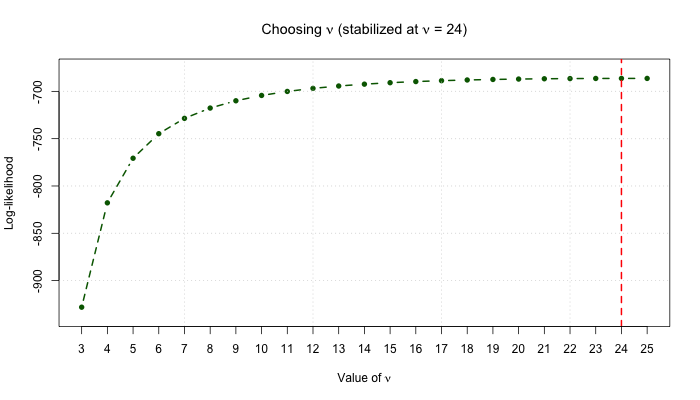
\includegraphics[scale=0.65]{ps6_plot5.png}
\end{center}

\end{document}
